\documentclass[11pt]{article}

\usepackage[margin=1in]{geometry}
\usepackage[T1]{fontenc}
\usepackage[utf8]{inputenc}
\usepackage{lmodern}
\usepackage{microtype}
\usepackage{graphicx}
\usepackage{booktabs}
\usepackage{longtable}
\usepackage{array}
\usepackage{amsmath,amssymb,amsthm}
\usepackage{enumitem}
\usepackage{xcolor}
\usepackage{hyperref}
\usepackage{url}
\usepackage{float}
\usepackage{caption}

\hypersetup{
  colorlinks=true,
  linkcolor=blue!50!black,
  citecolor=blue!50!black,
  urlcolor=blue!50!black
}

\newtheorem{proposition}{Proposition}
\newtheorem{definition}{Definition}

\newcommand{\paperid}{P1\_Contracts}
\newcommand{\validator}{\textsc{CoordinationContractValidator}}
\newcommand{\allow}{\texttt{allow}}
\newcommand{\deny}{\texttt{deny}}
\newcommand{\nongoals}{This paper does not claim Byzantine tolerance, partition-safe consensus, or live cross-transport deployment equivalence.}

\title{\textbf{Coordination Contracts: Trace-Derived Admission for Shared CPS State}}
\author{Anonymous authors\\
\small Replace with author names and affiliations for camera-ready}
\date{}

\begin{document}
\maketitle

\begin{abstract}
In cyber-physical systems (CPS), correct messaging does not imply correct coordination. A workflow may deliver every packet and still admit split-brain ownership conflicts, stale writes, reorder-sensitive violations, or out-of-scope updates to shared state. We present \emph{Coordination Contracts}, a portable coordination-admission semantics for shared keyed state that combines keyed authority, temporal admissibility, reason-coded denials, and trace-derivability at the write boundary. The key design constraint is \emph{trace-derivability}: verdicts must be reproducible from event traces plus declared configuration alone, without privileged hidden state. On the current benchmark artifact (54-sequence challenge corpus), the full contract matches the expected per-event verdict vector on all sequences and achieves event-level precision/recall/F1 of 1.0 (TP=37, FP=0, FN=0). Comparator decomposition shows that temporal-only proxies miss split-brain failures, while authority-only proxies miss stale and reorder-sensitive failures; the full contract improves over timestamp-only baselines by 13 denied violations. Validation overhead remains bounded in this trace-driven single-process setting, with event-level median/p95/p99 latency of 4.6/11.8/84.5~$\mu$s and bootstrap confidence intervals reported in the artifact. We also demonstrate transport-boundary semantic parity across event-log and LADS-shaped ingestion paths for canonical sequences. Optional async stress sweeps characterize sensitivity to delay, skew, and reorder; they support robustness discussion but do not replace the headline corpus verdict. \nongoals
\end{abstract}

\section{Introduction}

Communication is not coordination. In CPS orchestration, the correctness-critical question is not whether a message arrived, but whether a proposed write is admissible under explicit authority and temporal rules for shared keyed state.

\paragraph{Motivating vignette.}
Controller A releases a functional unit after finishing a task. Controller B, operating on stale assignment state, issues a new write on the same key. Transport delivery succeeds. Coordination still fails unless a shared-state admission layer denies the write. Coordination Contracts make this failure explicit at the write boundary with reason codes (e.g., \texttt{split\_brain}, \texttt{stale\_write}) before state mutation.

This paper proposes Coordination Contracts as a reusable coordination-admission layer above transport and below application policy. The model defines typed state, keyed authority, temporal admissibility, and transition validity. A pure validator consumes replay state and event fields and returns \allow/\deny with reason codes. \nongoals We instead claim something narrower and, we argue, practically valuable: a portable semantics layer that makes shared-state mutation auditable, replayable, and denyable under explicit authority and time rules.

\paragraph{Why now.}
Regulated CPS programs increasingly require post-incident traceability, evidence-preserving change control, and cross-team interoperability between heterogeneous controllers. A trace-derived admission layer is useful in this setting because it yields replayable enforcement decisions with explicit denial reasons, even when messaging succeeds.

The paper makes four claims:
\begin{enumerate}[leftmargin=1.5em]
\item A trace-derived validator can detect and deny the specified coordination failure classes on the benchmark corpus.
\item Validation is reproducible from traces plus declared configuration without privileged hidden state.
\item The model is transport-agnostic by construction at the event/state boundary; parity is shown for reference ingestion paths.
\item Per-write validation overhead is bounded on the evaluated workload.
\end{enumerate}

\section{Related work and positioning}

Contract Net introduced higher-level coordination semantics for distributed task sharing \cite{smith1980contract}. TLA$+$ provides a strong foundation for formal specification of concurrent and distributed systems \cite{lamport2002specifying}. ROS~2 and DDS provide transport, discovery, and data-centric publish-subscribe semantics for robotic and distributed applications \cite{ros2dds,ros2qos,ros2security}. Log-based systems such as Kafka provide durable replay and keyed retention \cite{kafkaIntro,kafkaCompact}. Classic optimistic concurrency and lease protocols address contention and stale ownership windows in distributed settings \cite{kung1981occ,gray1989leases}. OPC UA LADS provides rich laboratory information and orchestration-facing device semantics \cite{ladsScope,ladsIntro}.

Coordination Contracts are positioned differently: a portable write-validity layer for shared keyed state that combines explicit keyed authority, temporal admissibility, reason-coded denials, trace-derivability, and boundary-level transport portability. The goal is not to replace transport, industrial information models, or formal protocol methods. It is to make coordination admissibility auditable and replayable at the boundary where shared-state mutation is decided. In this sense, the paper argues for a missing systems layer: transport decides delivery, storage decides persistence, and coordination contracts decide whether a shared-state mutation is admissible.

This distinction is also what separates the present contribution from simpler reductions to timestamps, locks, or schema checks. Timestamp-only reasoning is insufficient for ownership conflicts; ownership-only reasoning is insufficient for stale or reorder-sensitive writes. Likewise, a device information model can describe state without deciding whether a candidate write is valid under explicit multi-writer authority and time rules. The paper's novelty is therefore in the combination, not in any one ingredient considered in isolation.

\paragraph{Positioning against adjacent mechanisms.}
Ordering policies, optimistic concurrency, leases, and locks address overlapping but distinct concerns: they govern \emph{when} a write may proceed under a particular concurrency protocol, not necessarily whether the write is admissible under an explicit multi-writer authority model for shared keyed state. Consensus and distributed transactions provide stronger guarantees under assumptions (membership, failure models, transactional boundaries) that this work does not adopt. This is not baseline emulation; it is boundary ingredient isolation. Coordination Contracts provide a lightweight, trace-replayable admission predicate at the write boundary, complementary to those mechanisms.

\section{Problem setting and failure model}

We consider multiple writers updating shared keyed state in CPS.

\paragraph{Failure classes.}
\begin{enumerate}[leftmargin=1.5em]
\item \textbf{Split-brain ownership conflict:} concurrent incompatible writers on one key.
\item \textbf{Stale write:} write based on outdated temporal state.
\item \textbf{Reorder-sensitive violation:} delayed/reordered writes violating declared acceptance order.
\item \textbf{Unknown-key access:} update outside declared contract scope.
\end{enumerate}

In the evaluated artifact, temporal ordering is reflected in per-event timestamps and the validator's monotonicity rules over admitted prefixes; reordering is modeled by permuting delivery order in corpus sequences while holding the same event fields.

\paragraph{Assumptions.}
Identity fields in traces are treated as truthful in this artifact. Validation occurs before mutation. The evaluated harness is trace-driven and single-process. We make no live deployment guarantees under Byzantine actors, network partitions, or arbitrary runtime interleavings beyond those reflected in the benchmark and auxiliary stress artifacts.

\section{Contract model and validator semantics}

\begin{definition}[Contract state]
For each key $k$, contract state stores typed value $v_k$, owner $o_k$, temporal summary $\tau_k$, and optional lease metadata $\ell_k$.
\end{definition}

\begin{definition}[Trace-derivability]
A validator is trace-derived if verdicts depend only on replay state from admitted prefix, event fields, and declared configuration $C$.
\end{definition}

The validator interface is:
\[
V_C(S,e)\rightarrow (\allow \mid \deny, R),
\]
where $R$ is a reason-code set.

\paragraph{Notation summary.}
$S$ denotes replay state reconstructed from admitted events; $e$ denotes the candidate event; $C$ denotes declared contract configuration; $R$ denotes reason-code output; $o_k$ denotes owner for key $k$; and $\tau_k$ denotes per-key temporal summary used for monotonicity checks.

\begin{proposition}[Determinism]
For fixed $C$, $S$, and $e$, the validator returns a unique verdict and reason-code set.
\end{proposition}

\begin{proposition}[Admitted-prefix invariants, sketch]
Let state evolve by applying only events with verdict \allow. Then ownership consistency and per-key temporal monotonicity are preserved along admitted prefixes under the declared contract predicates.
\end{proposition}

\noindent\emph{Scope note.}
The determinism property is aligned with the Lean formalization in \texttt{formal/lean/*/W2Contract.lean} (validator interface and trace-shaped reasoning); admitted-prefix invariants are presented as a proof sketch here and are not claimed as a complete mechanized proof of live distributed execution.

\paragraph{Worked example.}
Suppose the admitted prefix already records owner \texttt{controller\_a} for key \texttt{t1}. A candidate \texttt{task\_start} from \texttt{controller\_b} on \texttt{t1} yields verdict \deny{} with reason \texttt{split\_brain} because authority and ownership predicates fail. State is unchanged. If instead the candidate is a stale \texttt{task\_end} whose timestamp violates monotonicity, the verdict is \deny{} with \texttt{stale\_write} (or related temporal reason codes in the artifact). This makes coordination failure explicit before application of the write.

\section{Reference implementation and interoperability boundary}

The reference system separates a pure validator from a contract-enforcing store. Writes are applied only on \allow.

\begin{figure}[t]
\centering
\IfFileExists{figures/contracts_flow.pdf}{
  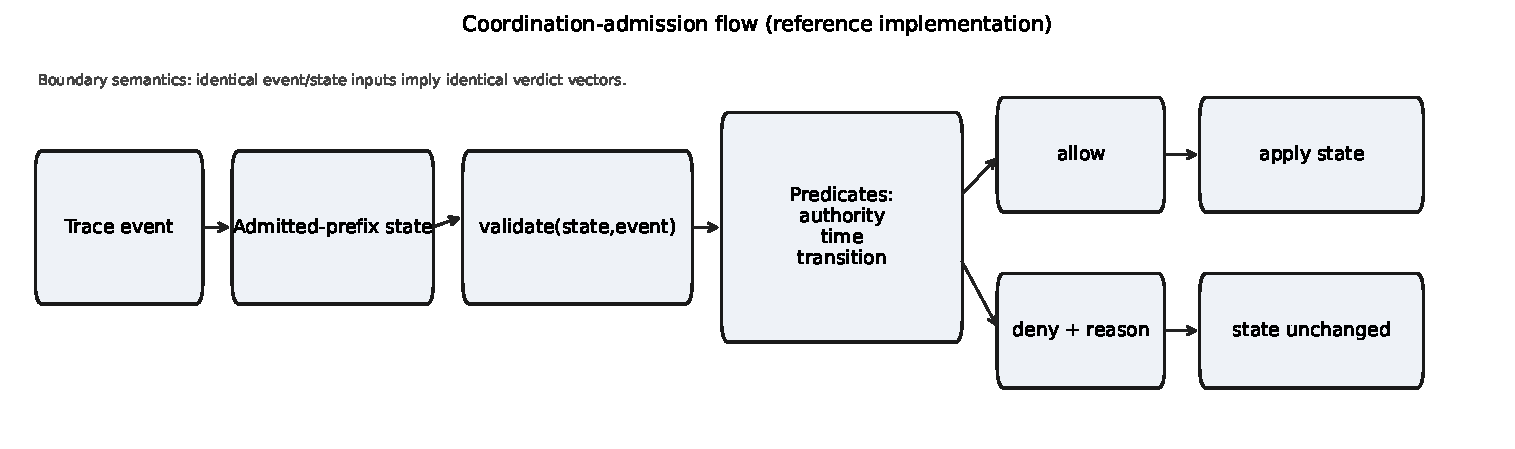
\includegraphics[width=0.92\linewidth]{figures/contracts_flow.pdf}
}{
  \fbox{\parbox[c][2.0in][c]{0.92\linewidth}{
  \centering
  Figure 0 placeholder: contract validation flow\\
  (replace with script-generated flow figure).
  }}
}
\caption{Coordination-admission flow. A candidate event passes through contract predicates and yields an \allow/\deny verdict with reason codes; state is updated only on \allow.}
\label{fig:flow}
\end{figure}

The transport claim is boundary scoped: if two ingestion paths induce identical event/state semantics at the contract boundary, they yield identical verdict vectors.

For OPC UA LADS-shaped interoperability, functional units or device-facing keys map to contract keys; controlling agents map to writers; LADS-compatible edges map to admissible transitions. The contract does not replace the LADS information model; it adds a portable admission check for writes alongside it.

\section{Experimental methodology}

\subsection{Benchmark corpus and metrics}

The current artifact evaluates a 54-sequence tiered corpus spanning positive controls, split-brain conflicts, stale writes, reorder-sensitive violations, unknown-key cases, and adversarial families such as cross-key interleaving, delayed release/reassignment, and concurrent controller races. Primary metric is exact per-event verdict-vector match per sequence. Secondary metrics include event-level TP/FP/FN, precision/recall/F1, class-level decomposition, event-level latency percentiles with bootstrap CIs, and boundary-level transport parity on canonical sequences.

\subsection{Ground truth and labeling}
Each sequence in \texttt{bench/contracts/corpus} carries an \texttt{expected\_verdicts} vector defined independently of any particular validator implementation (manual design with review, or generation with fixed seeds where applicable; see the benchmark specification). The evaluation checks that the contract's per-event verdict vector matches this ground truth. The corpus fingerprint and script version in \texttt{eval.json} identify the exact snapshot used for the tables in this paper.

\subsection{Failure-class inference and units of analysis}
Class-level slices in this paper are derived using deterministic sequence-family rules over sequence identifiers (e.g., names containing \texttt{split\_brain}, \texttt{stale}, \texttt{reorder}, \texttt{unknown}, with a control bucket for baseline-good/control families). We report three units of analysis: event-level metrics (TP/FP/FN and latency), sequence-level correctness (\texttt{detection\_ok}), and stress-profile-level sensitivity (\texttt{detection\_ok} rate under delay/skew/reorder settings).

\begin{table}[t]
\centering
\caption{Corpus composition by coarse family (from frozen run; heuristic family mapping over sequence identifiers).}
\label{tab:composition}
\begin{tabular}{lc}
\toprule
Family & Sequence count \\
\midrule
control & 14 \\
split\_brain & 9 \\
stale\_write & 8 \\
reorder & 7 \\
unknown\_key & 1 \\
other/adversarial/mixed & 15 \\
\bottomrule
\end{tabular}
\end{table}

\subsection{Comparator policies}

We evaluate:
\begin{itemize}[leftmargin=1.5em]
\item \texttt{full\_contract}
\item \texttt{timestamp\_only}
\item \texttt{ownership\_only}
\item \texttt{occ\_only} (reference proxy)
\item \texttt{lease\_only} (reference proxy)
\item \texttt{lock\_only} (reference proxy)
\item \texttt{naive\_lww}
\item \texttt{accept\_all}
\end{itemize}

\paragraph{Comparator caveat.}
OCC/lease/lock entries are benchmark proxies tied to available event fields; they are not full transaction-manager reimplementations. Their value is ingredient isolation at the coordination boundary: they show which semantic ingredients are necessary to deny the targeted failure classes, not how a production transaction manager would be engineered end to end.

\section{Results}

We organize results around the following questions: (RQ1) Does the full contract match ground truth on the benchmark? (RQ2) How do weaker comparators fail structurally? (RQ3) How do detection metrics decompose by inferred failure class? (RQ4) What is validation overhead in the evaluated harness? (RQ5) What does transport-boundary parity show? (RQ6) What does the async stress run characterize?

\subsection{RQ1: Exact match on the benchmark}

\begin{table}[t]
\centering
\caption{Core benchmark summary from \texttt{eval.json}. Exact match is measured over the full per-event verdict vector for each sequence.}
\label{tab:summary}
\begin{tabular}{lccccccc}
\toprule
Corpus & Seq. & Exact match & TP & FP & FN & Precision & Recall/F1 \\
\midrule
Tiered contracts corpus & 54 & 54/54 & 37 & 0 & 0 & 1.00 & 1.00 / 1.00 \\
\bottomrule
\end{tabular}
\end{table}

Table~\ref{tab:summary} answers RQ1: the contract matches the expected verdict vector on every sequence.

\subsection{RQ2: Structural failure of weaker policies}

\begin{table}[t]
\centering
\caption{Comparator decomposition from \texttt{ablation}. Entries report targeted violations denied versus missed under each policy. Policy names follow artifact identifiers.}
\label{tab:comparators}
\begin{tabular}{lcc}
\toprule
Policy & Denied & Missed \\
\midrule
\texttt{full\_contract} & 37 & 0 \\
\texttt{timestamp\_only} & 24 & 13 \\
\texttt{ownership\_only} & 20 & 17 \\
\texttt{occ\_only} & 24 & 13 \\
\texttt{lease\_only} & 24 & 13 \\
\texttt{lock\_only} & 20 & 17 \\
\texttt{naive\_lww} & 0 & 37 \\
\texttt{accept\_all} & 0 & 37 \\
\bottomrule
\end{tabular}
\end{table}

The structural pattern is stable and substantively important: temporal-only comparators miss split-brain conflicts; authority-only comparators miss stale and reorder-sensitive classes. This is the core empirical reason the paper should not be read as ``timestamps plus bookkeeping.'' The decisive behavior comes from combining authority and time semantics in one admission rule.
Compared to \texttt{timestamp\_only}, the full contract prevents 13 additional missed violations; compared to \texttt{ownership\_only}, it prevents 17 additional missed violations.

\paragraph{Comparator failure vignette.}
In split-brain sequences with concurrent claims on the same key, \texttt{timestamp\_only} and temporal proxies can accept conflicting ownership updates when timestamps are admissible, whereas authority-aware policies deny the second claim. Conversely, stale-write and reorder-sensitive sequences expose the weakness of ownership-only checks when temporal admissibility is omitted.

\begin{figure}[t]
\centering
\IfFileExists{../../docs/figures/p1_comparator_heatmap.png}{
  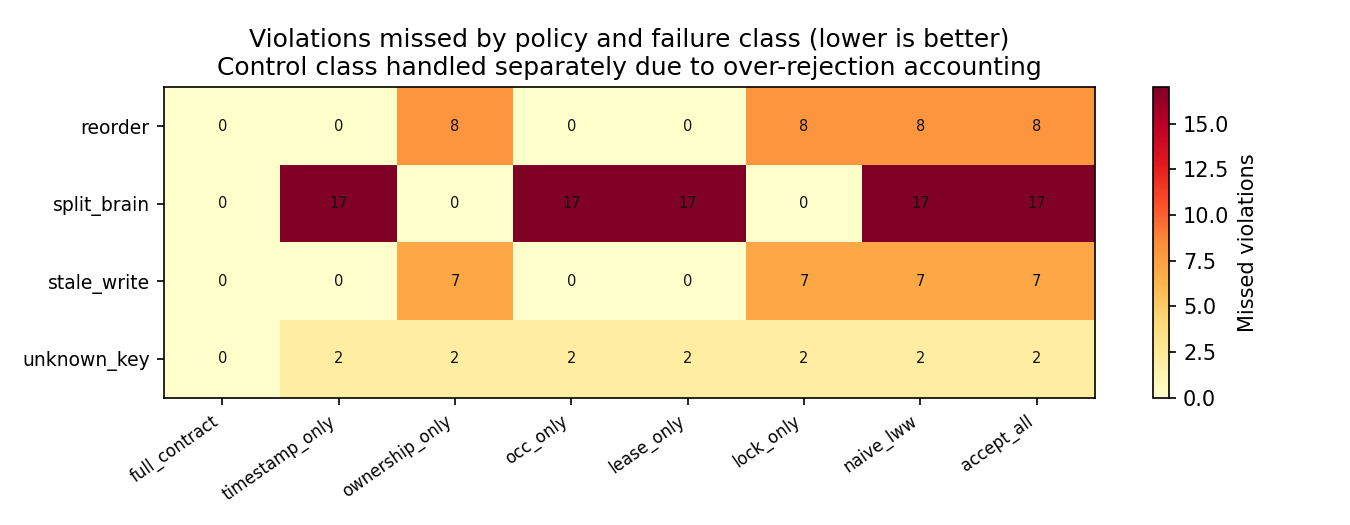
\includegraphics[width=\linewidth]{../../docs/figures/p1_comparator_heatmap.png}
}{
  \fbox{\parbox[c][1.8in][c]{0.92\linewidth}{\centering Placeholder: run \texttt{python scripts/plot\_p1\_paper\_figures.py}.}}
}
\caption{Violations \emph{missed} by policy and inferred failure class (darker is worse). Excludes the \texttt{control} class where negative ``missed'' counts indicate over-rejection in baseline accounting; see \texttt{ablation\_by\_class} in the artifact.}
\label{fig:heatmap}
\end{figure}

\begin{figure}[t]
\centering
\IfFileExists{../../docs/figures/p1_corpus_coverage.png}{
  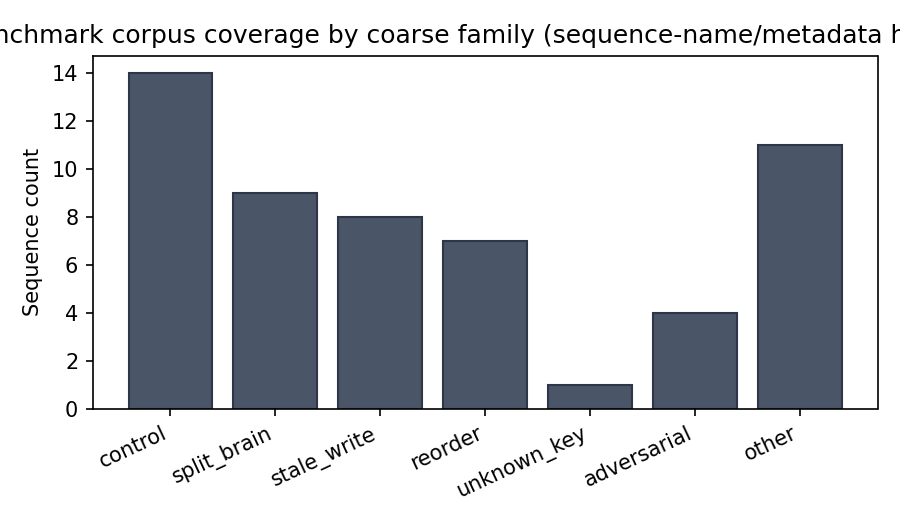
\includegraphics[width=0.82\linewidth]{../../docs/figures/p1_corpus_coverage.png}
}{
  \fbox{\parbox[c][1.5in][c]{0.82\linewidth}{\centering Placeholder: corpus coverage figure.}}
}
\caption{Corpus coverage by coarse family (heuristic from sequence name prefixes). Supplementary diversity is described in the corpus and appendix.}
\label{fig:coverage}
\end{figure}

\subsection{RQ3: Class-level diagnostics}

\begin{table}[t]
\centering
\caption{Detection metrics by inferred failure class from artifact field \texttt{detection\_metrics\_by\_class}.}
\label{tab:classmetrics}
\begin{tabular}{lcccccc}
\toprule
Class & TP & FP & FN & Precision & Recall & F1 \\
\midrule
control & 3 & 0 & 0 & 1.0 & 1.0 & 1.0 \\
reorder & 8 & 0 & 0 & 1.0 & 1.0 & 1.0 \\
split\_brain & 17 & 0 & 0 & 1.0 & 1.0 & 1.0 \\
stale\_write & 7 & 0 & 0 & 1.0 & 1.0 & 1.0 \\
unknown\_key & 2 & 0 & 0 & 1.0 & 1.0 & 1.0 \\
\bottomrule
\end{tabular}
\end{table}

\begin{table}[t]
\centering
\caption{Per-class detection-rate 95\% confidence intervals from artifact field \texttt{excellence\_metrics.per\_class\_ci95}.}
\label{tab:classci}
\begin{tabular}{lccc}
\toprule
Class & Rate & 95\% CI lower & 95\% CI upper \\
\midrule
control & 1.0 & 0.4385 & 1.0 \\
reorder & 1.0 & 0.6756 & 1.0 \\
split\_brain & 1.0 & 0.8157 & 1.0 \\
stale\_write & 1.0 & 0.6457 & 1.0 \\
unknown\_key & 1.0 & 0.3424 & 1.0 \\
\bottomrule
\end{tabular}
\end{table}

The perfect per-class scores should be read together with these interval widths. The benchmark result is strong, but the uncertainty bands remain wider for smaller classes such as \texttt{unknown\_key} and the control subset. This is exactly why the paper should frame the result as benchmark-backed evidence rather than as an unrestricted field-performance guarantee.
For \texttt{unknown\_key}, the wide interval reflects a small sample regime rather than weak observed performance; this class should be interpreted with caution.

\subsection{RQ4: Overhead and scale}

Event-level latency is bounded in this evaluated setting: median 4.6~$\mu$s, p95 11.8~$\mu$s, p99 84.5~$\mu$s, with bootstrap confidence intervals of [4.1, 5.4], [9.2, 27.2], and [19.1, 141.9]~$\mu$s respectively.

\begin{figure}[t]
\centering
\IfFileExists{../../docs/figures/p1_latency_percentiles.png}{
  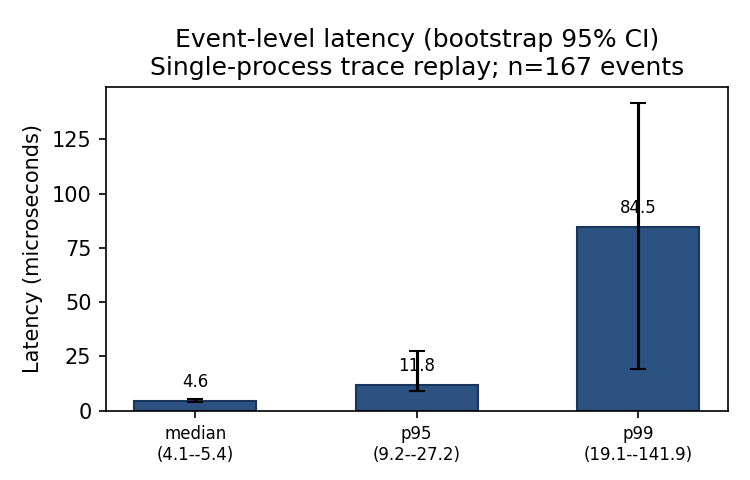
\includegraphics[width=0.88\linewidth]{../../docs/figures/p1_latency_percentiles.png}
}{
  \fbox{\parbox[c][1.8in][c]{0.88\linewidth}{\centering Placeholder: run \texttt{python scripts/plot\_p1\_paper\_figures.py}.}}
}
\caption{Event-level latency percentiles with bootstrap 95\% CIs (single-process trace replay; \texttt{latency\_percentiles\_us} in \texttt{eval.json}).}
\label{fig:latency}
\end{figure}

\begin{figure}[t]
\centering
\IfFileExists{../../docs/figures/p1_scale_throughput.png}{
  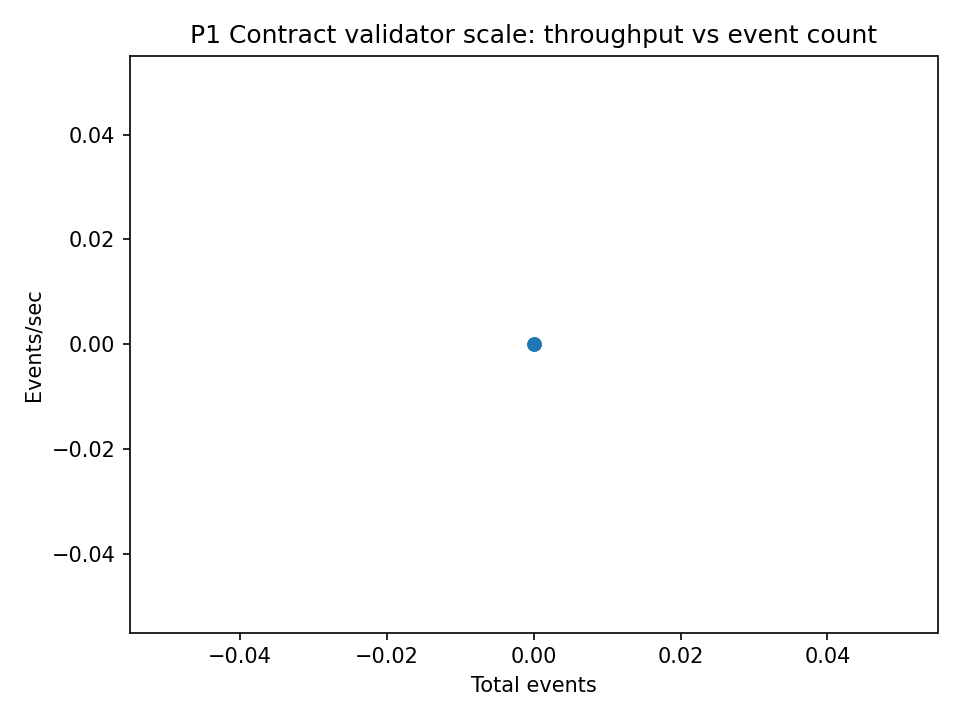
\includegraphics[width=0.88\linewidth]{../../docs/figures/p1_scale_throughput.png}
}{
  \fbox{\parbox[c][2.0in][c]{0.88\linewidth}{
  \centering
  Figure: scale throughput plot\\
  (replace with \texttt{docs/figures/p1\_scale\_throughput.png}).
  }}
}
\caption{Scale-throughput curve from the current P1 scale-test artifact. This figure is interpretive only: it characterizes the reference implementation in the evaluated single-process setting and should not be read as a deployment-wide performance guarantee.}
\label{fig:scale}
\end{figure}

\subsection{RQ5: Transport-boundary parity}

\begin{table}[t]
\centering
\caption{Boundary parity on canonical sequences from \texttt{transport\_parity.json}. `yes' denotes identical verdict vectors across the compared ingestion paths.}
\label{tab:parity}
\begin{tabular}{lcc}
\toprule
Sequence & Event count & Parity \\
\midrule
\texttt{good\_sequence} & 2 & yes \\
\texttt{split\_brain\_sequence} & 1 & yes \\
\texttt{reorder\_sequence} & 2 & yes \\
\texttt{actor\_payload\_writer\_mismatch} & 1 & yes \\
\bottomrule
\end{tabular}
\end{table}

All canonical parity checks pass (\texttt{parity\_ok\_all=true}; parity rate 1.0 over 6/6 checked events). This supports boundary semantic consistency only; it is not a claim of end-to-end transport equivalence across full runtime stacks.

\subsection{RQ6: Async stress characterization}

The artifact includes an async stress runner that sweeps delay, clock-skew, and reorder profiles. We treat this as robustness characterization, not as a substitute for the primary corpus evaluation. Figure~\ref{fig:stress} summarizes detection retention by profile when \texttt{stress\_results.json} is present; the main correctness claim remains anchored in RQ1. Sensitivity is dominated by profile-induced reordering and timestamp perturbation rather than by pure delay in isolation.

\begin{figure}[t]
\centering
\IfFileExists{../../docs/figures/p1_stress_summary.png}{
  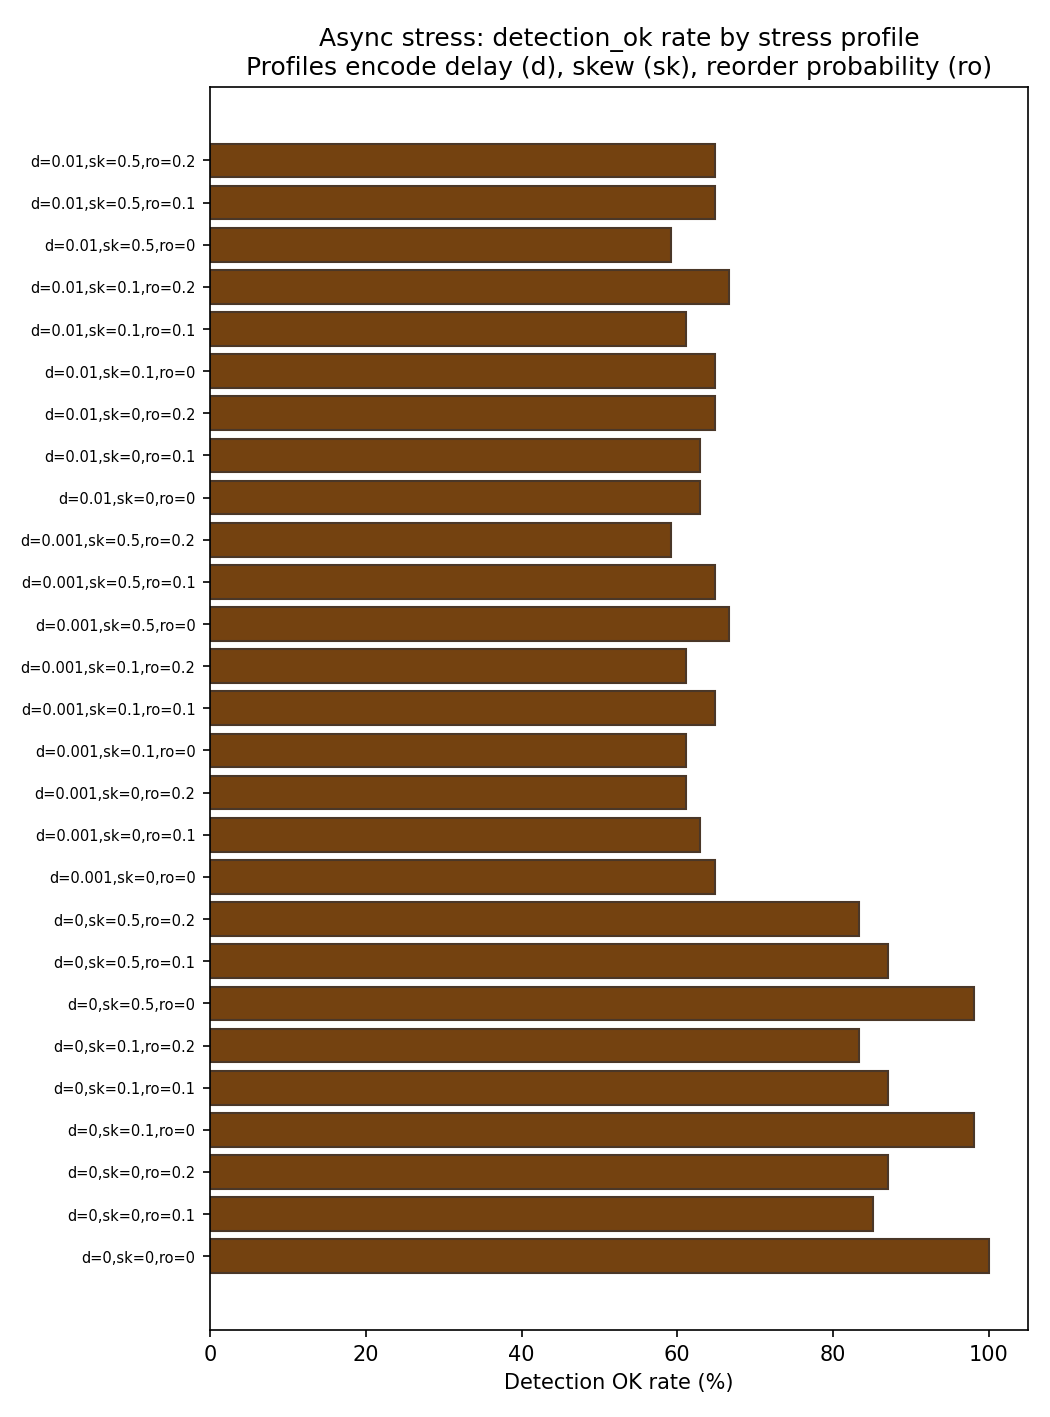
\includegraphics[width=\linewidth]{../../docs/figures/p1_stress_summary.png}
}{
  \fbox{\parbox[c][1.5in][c]{0.92\linewidth}{\centering Placeholder: run \texttt{contracts\_async\_stress.py} then \texttt{plot\_p1\_paper\_figures.py}.}}
}
\caption{Async stress: fraction of runs with \texttt{detection\_ok} true, by stress profile (see \texttt{stress\_results.json}). Interpret as sensitivity analysis, not field deployment.}
\label{fig:stress}
\end{figure}

\section{Discussion}

The key claim is not that transport can be ignored; it is that transport-level correctness and coordination-level admissibility are distinct. Coordination Contracts isolate that missing layer with explicit predicates and replayable evidence. This provides operational value in post-incident reconstruction, reproducible debugging, and explicit denial reasoning.

This replayability matters especially in regulated or safety-relevant workflows. If a deny is tied to explicit predicates and reason codes, an auditor can reconstruct why a write was rejected, distinguish transport success from coordination invalidity, and trace the decision back to the admitted-prefix state without privileged runtime metadata.

\section{Limitations and threats to validity}

\begin{itemize}[leftmargin=1.5em]
\item \textbf{Synthetic benchmark scope:} corpus is deliberate but synthetic.
\item \textbf{Corpus authorship:} sequences and expected verdicts are produced within the same benchmark release process; mitigate by frozen fingerprints, independent re-runs, and benchmark documentation of labeling rules.
\item \textbf{Single-process evaluation:} no live distributed deployment claims.
\item \textbf{Identity trust in trace fields:} Byzantine identity spoofing out of scope.
\item \textbf{Boundary-level transport claim:} parity is boundary semantics, not live-system equivalence.
\item \textbf{Comparator scope:} OCC/lease/lock are reference proxies in this corpus model.
\item \textbf{Stress interpretation scope:} async stress outputs characterize sensitivity under delay/skew/reorder profiles, but they do not substitute for multi-process or networked deployment evidence.
\item \textbf{Canonical non-goals:} \nongoals
\end{itemize}

\section{Conclusion}

Coordination Contracts provide a trace-derived admission layer for shared CPS state: explicit keyed authority, temporal admissibility, and reason-coded denials at the write boundary. On the current benchmark artifact, the approach matches expected verdict vectors across all corpus sequences with bounded per-write overhead in the evaluated setting, and its comparator decomposition shows why weaker policies fail. \nongoals The contribution is strongest when read as a reusable and auditable semantics layer with explicit limits, not as a surrogate for consensus, authentication, or full distributed-runtime verification.

\begin{thebibliography}{9}

\bibitem{smith1980contract}
Reid G. Smith.
\newblock The Contract Net Protocol: High-Level Communication and Control in a Distributed Problem Solver.
\newblock \emph{IEEE Transactions on Computers}, C-29(12):1104--1113, 1980.

\bibitem{lamport2002specifying}
Leslie Lamport.
\newblock \emph{Specifying Systems: The TLA+ Language and Tools for Hardware and Software Engineers}.
\newblock Addison-Wesley, 2002.

\bibitem{ros2dds}
S. Macenski, T. Foote, B. Gerkey, C. Lalancette, and W. Woodall.
\newblock Robot Operating System 2: Design, architecture, and uses in the wild.
\newblock \emph{Science Robotics}, 7(66):eabm6074, 2022.

\bibitem{ros2qos}
G. Pardo-Castellote.
\newblock OMG Data-Distribution Service: Architectural overview.
\newblock In \emph{Proceedings of the 23rd International Conference on Distributed Computing Systems Workshops}, 2003.

\bibitem{ros2security}
V. Mayoral Vilches, R. White, G. Caiazza, and M. Arguedas.
\newblock SROS2: Usable cyber security tools for ROS 2.
\newblock In \emph{2022 IEEE/RSJ International Conference on Intelligent Robots and Systems (IROS)}, 2022.

\bibitem{kafkaIntro}
J. Kreps, N. Narkhede, and J. Rao.
\newblock Kafka: A distributed messaging system for log processing.
\newblock In \emph{Proceedings of the NetDB Workshop}, 2011.

\bibitem{kafkaCompact}
Apache Kafka Documentation.
\newblock Topic configuration: \texttt{cleanup.policy}.
\newblock Accessed March 2026.

\bibitem{kung1981occ}
H. T. Kung and J. T. Robinson.
\newblock On optimistic methods for concurrency control.
\newblock \emph{ACM Transactions on Database Systems}, 6(2):213--226, 1981.

\bibitem{gray1989leases}
C. Gray and D. Cheriton.
\newblock Leases: An efficient fault-tolerant mechanism for distributed file cache consistency.
\newblock In \emph{Proceedings of the Twelfth ACM Symposium on Operating Systems Principles}, pages 202--210, 1989.

\bibitem{ladsScope}
OPC Foundation.
\newblock OPC 30500-1: Laboratory and Analytical Devices.
\newblock Version 1.00, 2025.

\bibitem{ladsIntro}
OPC Foundation.
\newblock Laboratory and Analytical Devices: General information on LADS and OPC UA.
\newblock Version 1.00, 2025.

\end{thebibliography}

\appendix

\section{Reproducibility block}

From repository root:
\begin{enumerate}[leftmargin=1.5em]
\item \texttt{PYTHONPATH=impl/src python scripts/contracts\_eval.py --out datasets/runs/contracts\_eval}
\item \texttt{PYTHONPATH=impl/src python scripts/contracts\_transport\_parity.py --out datasets/runs/contracts\_eval}
\item \texttt{python scripts/export\_contracts\_corpus\_table.py --eval datasets/runs/contracts\_eval/eval.json}
\item \texttt{python scripts/export\_p1\_appendix\_tex.py --eval datasets/runs/contracts\_eval/eval.json}
\item \texttt{python scripts/export\_p1\_contract\_flow.py}
\item \texttt{python scripts/render\_p1\_flow\_figure.py}
\item \texttt{python scripts/plot\_contracts\_scale.py}
\item \texttt{python scripts/plot\_p1\_paper\_figures.py --eval datasets/runs/contracts\_eval/eval.json}
\item \texttt{PYTHONPATH=impl/src python scripts/contracts\_async\_stress.py --out datasets/runs/contracts\_eval} (optional; produces \texttt{stress\_results.json})
\end{enumerate}

The run used for this draft should record \texttt{run\_manifest.script\_version}, \texttt{run\_manifest.corpus\_fingerprint}, and \texttt{run\_manifest.corpus\_sequence\_count} in \texttt{eval.json}. One-shot generation: \texttt{python scripts/generate\_paper\_artifacts.py --paper P1}.

\section{Full per-sequence corpus summary}

\IfFileExists{generated_appendix_corpus.tex}{
% Auto-generated by scripts/export_p1_appendix_tex.py — do not edit by hand.
% Regenerate: python scripts/export_p1_appendix_tex.py --eval <path/to/eval.json>

\begin{longtable}{p{0.52\linewidth}cc}
\caption{Per-sequence corpus summary (frozen run).}\label{tab:appendixcorpus}\\
\toprule
Sequence & Detection OK & Contract denials \\
\midrule
\endfirsthead
\toprule
Sequence & Detection OK & Contract denials \\
\midrule
\endhead
actor\_payload\_writer\_mismatch & yes & 1 \\
burst\_duplicate\_three & yes & 0 \\
concurrent\_controller\_race & yes & 2 \\
conflicting\_writes\_independent\_keys & yes & 0 \\
coordination\_message\_passthrough & yes & 0 \\
cross\_key\_interleaved\_race & yes & 0 \\
delayed\_release\_reassignment & yes & 1 \\
duplicate\_delivery & yes & 0 \\
edge\_case\_timestamps & yes & 0 \\
good\_eight\_events & yes & 0 \\
good\_five\_events & yes & 0 \\
good\_four\_events & yes & 0 \\
good\_interleaved\_6 & yes & 0 \\
good\_sequence & yes & 0 \\
good\_sequence\_4events & yes & 0 \\
good\_seven\_events & yes & 0 \\
good\_single\_allow & yes & 0 \\
good\_six\_keys & yes & 0 \\
good\_ten\_events & yes & 0 \\
good\_then\_unknown\_key & yes & 1 \\
good\_three\_events & yes & 0 \\
good\_three\_keys\_cycle & yes & 0 \\
good\_two\_keys & yes & 0 \\
long\_horizon\_10 & yes & 0 \\
mixed\_key\_contention\_8 & yes & 0 \\
multi\_key\_no\_conflict & yes & 0 \\
multi\_writer\_contention & yes & 1 \\
reorder\_burst\_four & yes & 1 \\
reorder\_first\_deny & yes & 1 \\
reorder\_first\_event\_deny & yes & 1 \\
reorder\_mid\_chain & yes & 1 \\
reorder\_multi\_key & yes & 1 \\
reorder\_sequence & yes & 1 \\
reorder\_three\_events & yes & 1 \\
same\_ts\_same\_writer & yes & 0 \\
split\_brain\_delayed\_conflict & yes & 1 \\
split\_brain\_five\_writers & yes & 4 \\
split\_brain\_four\_writers & yes & 3 \\
split\_brain\_same\_epoch & yes & 1 \\
split\_brain\_second\_key & yes & 1 \\
split\_brain\_sequence & yes & 1 \\
split\_brain\_then\_allow & yes & 1 \\
split\_brain\_three\_writers & yes & 2 \\
split\_brain\_two\_keys & yes & 1 \\
stale\_then\_allow & yes & 1 \\
stale\_write\_delayed\_delivery & yes & 1 \\
stale\_write\_exact & yes & 0 \\
stale\_write\_margin & yes & 1 \\
stale\_write\_sequence & yes & 1 \\
stale\_write\_sequence\_2 & yes & 1 \\
stale\_write\_sequence\_3 & yes & 1 \\
stale\_write\_sequence\_4 & yes & 1 \\
unknown\_key\_deny & yes & 1 \\
unsafe\_lww\_sequence & yes & 1 \\
\bottomrule
\end{longtable}

\paragraph{Run manifest (reproducibility).} Script version \texttt{v0.3}; corpus fingerprint \texttt{ae76bbcc00c1b194}; sequence count 54.

}{
\textit{Regenerate appendix table:} \texttt{python scripts/export\_p1\_appendix\_tex.py --eval <path/to/eval.json>}
}

\section{How to regenerate main-text numbers}
\begin{itemize}[leftmargin=1.5em]
\item Table~\ref{tab:summary}, Table~\ref{tab:comparators}, Table~\ref{tab:classmetrics}, Table~\ref{tab:classci}: from \texttt{datasets/runs/contracts\_eval/eval.json}.
\item Table~\ref{tab:parity}: from \texttt{datasets/runs/contracts\_eval/transport\_parity.json}.
\item Figures~\ref{fig:heatmap}, \ref{fig:coverage}, \ref{fig:latency}, \ref{fig:stress}: \texttt{python scripts/plot\_p1\_paper\_figures.py --eval <eval.json> [--stress <stress\_results.json>]}.
\item Figure~\ref{fig:flow}: \texttt{python scripts/render\_p1\_flow\_figure.py}.
\item Figure~\ref{fig:scale}: \texttt{python scripts/plot\_contracts\_scale.py}.
\end{itemize}

\section{Artifact schema snippets}
\paragraph{\texttt{eval.json} (key fields).}
\texttt{run\_manifest\{script\_version, corpus\_fingerprint, corpus\_sequence\_count\}}, \texttt{sequences[]}, \texttt{ablation}, \texttt{ablation\_by\_class}, \texttt{detection\_metrics\_by\_class}, \texttt{latency\_percentiles\_us}, \texttt{excellence\_metrics}.

\paragraph{\texttt{transport\_parity.json} (key fields).}
\texttt{parity\_ok\_all}, \texttt{per\_sequence[]}, \texttt{parity\_confidence\{matching\_events,total\_events\_checked,parity\_rate\}}.

\paragraph{\texttt{stress\_results.json} (key fields).}
\texttt{stress\_sweep}, \texttt{results[]\{sequence,stress\_profile,detection\_ok,latency\_stats\}}, \texttt{run\_manifest\{delay\_sweep,skew\_sweep,reorder\_probs,seed\}}.

\section{Proxy comparator limits}
\begin{itemize}[leftmargin=1.5em]
\item \texttt{occ\_only}, \texttt{lease\_only}, and \texttt{lock\_only} are benchmark proxies over available event fields.
\item They do not model full read sets, lease renewal windows, or lock-acquisition protocols.
\item Their purpose is boundary ingredient isolation, not production-equivalent transaction manager emulation.
\end{itemize}

\section{Threats-to-reproducibility checklist}
\begin{itemize}[leftmargin=1.5em]
\item Freeze and report \texttt{run\_manifest} values in cited artifacts.
\item Regenerate all figures/tables from the same run directory before submission.
\item Record Python and plotting backend versions when exporting figures.
\item Ensure no placeholder figure/table remains in the compiled manuscript.
\end{itemize}

\section{Reviewer-objection map}
\begin{itemize}[leftmargin=1.5em]
\item \textbf{``Baselines are weak.''} Addressed by explicit proxy caveat and class-level comparator decomposition.
\item \textbf{``Synthetic benchmark overfits.''} Addressed by anti-circular labeling governance, frozen manifests, and per-sequence appendix reporting.
\item \textbf{``Transport claim is too broad.''} Addressed by boundary-only parity wording and explicit non-goals.
\item \textbf{``Where is full formal proof?''} Addressed by Lean-aligned determinism scope and explicit proof-sketch boundaries.
\end{itemize}

\end{document}
